\chapter{Терминология}

\section{Конвейер}

\noindent Конвейер -- средство непрерывной перевозки ресурсов между двумя любыми точками.

\

\noindent Каждый конвейер характеризуется:
\begin{itemize}
	\item Формой
	
		Описывается системой уравнений:
		$$\vec{r}(t) = \begin{cases} x_1 = x_1(t) \\ \vdots \\ x_n = x_n(t) \\ \end{cases} \subseteq \ \mathbb{R}^n$$
		В частности: $\mathbb{R}^3$ (Satisfactory) или $\mathbb{R}^2$ (Factoro)
	
	\item Функцией распределения динамики скорости вдоль конвейера 
		
		$v(\vec{r}, t) \cong v(t_{\text{path}}, t_{\text{time}}) = v\left(\vec{t}\right)$
	
	\item Начальной $\vec{r}(0)$ и конечной $\vec{r}(t\to\text{max})$ точкой
\end{itemize}


\vspace{0.3in}


На чертежах обозначается кривой, либо отрезком, соединяющим пару точек. Может иметь стрелки для указания направления движения, а рядом может подписываться пропускная способность:

\vspace{0.5in}


\begin{tikzpicture}[
	s/.style={rectangle, draw=black!60, fill=black!5, thin, minimum size=20},
	a/.style={rectangle, draw=black!60, fill=black!5, thin, minimum size=20},
	o/.style={rectangle, draw=black!60, fill=black!5, thin, minimum size=20},
	]
	
	%Nodes
	\node[a]    (a1)                          	{a};
	\node[s]    (s1)        [above = of a1]     {s};
	\node[s]    (s2)        [left = of s1]      {s};
	\node[o]	(in1)		[below = of a1]		{in};
	\node[a]    (a2)        [above = of s1]   	{a};
	\node[o]	(out1)		[above = of a2]		{out};
	\node[o]	(out2)		[left = of out1]	{out};
	
	%Lines
	\draw[->, ultra thick] (in1.north) to node[right] 	 			 {$\boldmath{ 1 }$} 		  (a1.south);
	\draw[->, ultra thick] (a1.north)  to node[right] 	 		 	 {$\boldmath{ \frac{6}{5} }$} (s1.south);
	\draw[->, ultra thick] (s1.west)   to node[above] 	 		 	 {$\boldmath{ \frac{2}{5} }$} (s2.east);
	\draw[->, ultra thick] (s2) 	   to[bend left=-45] node[left]  {$\boldmath{ \frac{1}{5} }$} (a1);
	\draw[->, ultra thick] (s1.north)  to node[right] 				 {$\boldmath{ \frac{2}{5} }$} (a2.south);
	\draw[->, ultra thick] (s1) 	   to[bend right=90] node[right] {$\boldmath{ \frac{2}{5} }$} (a2);
	\draw[->, ultra thick] (a2.north)  to node[right] 	 			 {$\boldmath{ \frac{4}{5} }$} (out1.south);
	\draw[->, ultra thick] (s2.north)  to node[left]	 			 {$\boldmath{ \frac{1}{5} }$} (out2.south);
\end{tikzpicture}






\newpage

\section{Конвейерный разъединитель}

\

Конвейерный разъединитель (англ: splitter) -- устройство, разъединяющее одну конвейерную ленту на несколько других.

\

\noindent Каждый конвейерный разъединитель характеризуется:

\begin{itemize}
	\item числом выходных лент $n \in \mathbb{N}$
	
	\item правилами вывода: $\{ \varphi_i \}$
\end{itemize}

\vspace{0.15in}

%На чертежах обозначается фигурой (обычно, квадрат) с буквой "s" (splitter), к которому с одной стороны подводится конвейер, а с остальных сторон -- конвейеры отводятся:
%Будем обозначать фигурой синего цвета, а буквой (s, или f характеризовать конвкретный тип), а на выходах специальными метками обозначать правило $\varphi_i$.
На чертежах обозначается синей фигурой (обычно, квадрат). Буква внутри ("s" -- splitter, "f" -- filter, итд) характеризует подтип устройства. На выходах могут находиться специальные метки, обозначающие правила вывода $\varphi_i$. К разъединителю с одной стороны подводится конвейер, а со всех остальных -- конвейеры отводятся.


\vspace{0.4in}


\begin{minipage}{0.3\textwidth}
	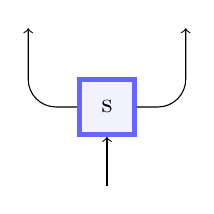
\begin{tikzpicture}[
		s/.style={rectangle, draw=blue!60, fill=blue!5, ultra thick, minimum size=20},
		r/.style = {->, thin, rounded corners=10pt},
		]
		
		\node[s]    (s)		at	(0, 0)	{s};
		\draw[r]	(0,-1)	to	(s);
		\draw[r]	(s)		-|	(-1, 1);
		\draw[r]	(s)		-|	(1, 1);
	\end{tikzpicture}
\end{minipage}
\begin{minipage}{0.3\textwidth}
	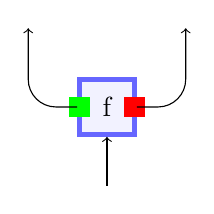
\begin{tikzpicture}[
		s/.style = {rectangle, draw=blue!60,	fill=blue!5,	ultra thick, minimum size=20},
		a/.style = {rectangle, draw=black!60,	fill=black!5,		  thin,  minimum size=20},
		o/.style = {rectangle, draw=black!60,	fill=black!5,		  thin,  minimum size=20},
		q/.style = {rectangle, draw,			fill, 						 minimum size=0.25cm},
		r/.style = {->, thin, rounded corners=10pt},
		l/.style = {	thin, rounded corners=10pt},
		]
		
		
		% === === Nodes === ===
		\node[s]		(f)		at	(0, 0)			{f};
		\node[q, red]	(n3)	at	(0.35, 0)		{};
		\node[q, green]	(n4)	at	(-0.35, 0)		{};
		
		\draw[r]		(f)		-|	(-1, 1);
		\draw[r]		(f)		-|	(1, 1);
		\draw[r]		(0, -1)	to	(f);
		
	\end{tikzpicture}
\end{minipage}

















\vspace{0.5in}

\section{Конвейерный соединитель}

\

Конвейерный соединитель (англ: adder/merger) -- устройство, соединяющее несколько входных лент в одну.

\

\noindent Каждый конвейерный соединитель характеризуется

\begin{itemize}
	\item Числом входных лент $n \in \mathbb{N}$
	
	\item Правилами приёма(ввода): $\{ \varphi_i \}$
\end{itemize}


\vspace{0.15in}

%На чертежах обозначается фигурой (обычно, квадратом) с буквой "a" (adder), к которому с одной стороны подводится конвейер на вывод, а с остальных сторон -- конвейеры входят:
На чертежах обозначается красной фигурой (обычно, квадрат). Буква внутри ("a" -- adder, "p" -- priority, итд) характеризует подтип устройства. На входах могут находиться специальные метки, обозначающие правила ввода $\varphi_i$. От соединителя с одной стороны конвейер отводится, а к остальным -- подводятся.


\vspace{0.4in}


\begin{minipage}{0.3\textwidth}
	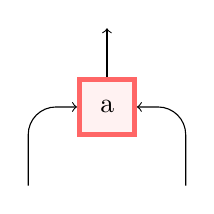
\begin{tikzpicture}[
		a/.style={rectangle, draw=red!60, fill=red!5, ultra thick, minimum size=20},
		r/.style = {->, thin, rounded corners=10pt},
		]
		
		%Nodes
		\node[a]    (a)			at	(0, 0)	{a};
		\draw[r]	(-1, -1)	|-	(a);
		\draw[r]	(1, -1)		|-	(a);
		\draw[r]	(a)			to	(0, 1);
	\end{tikzpicture}
\end{minipage}
\begin{minipage}{0.3\textwidth}
	\begin{tikzpicture}[
		a/.style={rectangle, draw=red!60, fill=red!5, ultra thick, minimum size=20},
		r/.style = {->, thin, rounded corners=10pt},
		]
		
		
		\node[
			draw=red!60, fill=red!5, very thick,
			regular polygon, regular polygon sides=3, 
			rotate=-90, minimum size=0.5cm
			] 
					(tri)	at  (-0.4, 0) {};
		\node[a]	(p)		at	(0, 0)			{p};
		\node				at	(-0.45, 0)		{$1$};
		
		\draw[r]	(-1, -1)	|-	(tri);
		\draw[r]	(1, -1)		|-	(p);
		\draw[r]	(p)			to	(0, 1);
	\end{tikzpicture}
\end{minipage}
\begin{minipage}{0.3\textwidth}
	\begin{tikzpicture}[
		a/.style={rectangle, draw=red!60, fill=red!5, ultra thick, minimum size=20},
		r/.style = {->, thin, rounded corners=10pt},
		]
		
		
		\node[
			draw=red!60, fill=red!5, very thick,
			regular polygon, regular polygon sides=3, 
			rotate=-90, minimum size=0.5cm
			] 
					(tri1)	at  (-0.4, 0) {};
		\node				at	(-0.45, 0)		{$3$};
		
		\node[
			draw=red!60, fill=red!5, very thick,
			regular polygon, regular polygon sides=3, 
			rotate=90, minimum size=0.5cm
			] 
					(tri2)	at  (0.4, 0) {};
		\node				at	(0.45, 0)		{$5$};
		
		\node[a]	(p)		at	(0, 0)			{:};
		
		\draw[r]	(-1, -1)	|-	(tri1);
		\draw[r]	(1, -1)		|-	(tri2);
		\draw[r]	(p)			to	(0, 1);
	\end{tikzpicture}
\end{minipage}








\vspace{0.4in}

Также существуют специальные объекты, которые не являются ни соединителями ни разъединителями в прямом смысле: 
они как бы перемешивают ресурсы между конвейерами. Имеют они, соответственно по два входа и выхода:






\vspace{0.4in}

\begin{minipage}{0.315\textwidth}
	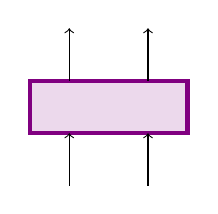
\begin{tikzpicture}[
		r/.style = {->, thin, rounded corners=10pt},
		]
		
		\draw[draw={rgb:red,255;blue,255},	fill={rgb:red!15,255;blue!15,255}, ultra thick]	(-1, 0.333)	rectangle node {$\rightleftarrows$} (1, -0.333);
		\draw[r]	(-0.5, -1)		to	(-0.5, -0.333);
		\draw[r]	(0.5, -1)		to	(0.5, -0.333);
		\draw[r]	(-0.5, 0.333)	to	(-0.5, 1);
		\draw[r]	(0.5, 0.333)	to	(0.5, 1);
	\end{tikzpicture}
\end{minipage}
\begin{minipage}{0.3\textwidth}
	\begin{tikzpicture}[
		s/.style = {rectangle, draw={rgb:red,255;blue,255},	fill={rgb:red!15,255;blue!15,255},	ultra thick, minimum size=20},
		r/.style = {->, thin, rounded corners=10pt},
		]
		
		
		% === === Nodes === ===
		\node[s]		(m)		at	(0, 0)			{m};
		\draw[draw=orange,	fill=orange, ultra thick]	(0.45, 0.333)	rectangle (0.5, -0.333);
		\node[
		draw=orange, fill=orange, very thick,
		regular polygon, regular polygon sides=3, 
		rotate=90, 
		minimum size=0.12cm, inner sep=0.12cm, outer sep=0.12cm,
		] 
		(tri1) at (-0.667, 0) 		{};
		
		\draw[r]	(0.5, -1)	to	(0.5, 1);
		\draw[r]	(-1, -1)	to	(-1, 1);
		
	\end{tikzpicture}
\end{minipage}






